\appendix
\setcounter{figure}{0}
\section{Details of experiment setting}
\label{apdx:detail}
Our test machine is equipped with an Intel i9-7920X CPU and two GTX1080Ti GPU. The operating system is Ubuntu 16.04 LTS and uses the configuration of python3.5.2 + torch0.4.1 + gym0.10.8 + mujoco-py1.50.1.62 + mujoco150.

We use a "number states - 64 - 64 - number action" mlp network as actor and "number states - 64+number action - 64 - 1" mlp network as critic. Both network use ReLU as non-linear function and a "softsign":$f(x)=\frac{x}{1+|x|}$ is used at actor' output to limit the output between $(-1,1)$. Both network use layer-norm before ReLU as normalization function.

All the environments has been constrained in 1000 time steps, it means that one episode cannot last more than 1000 time steps. We train the agent for 500 epochs and evaluated the actor without exploration strategy for 10 times to get mean return. In each epoch, the agent rollouts 100 steps in environment and stores them into replay buffer, then update critic and actor 50 iterations. More details on the training process can be obtained from open source code at github.com/anonymousforcodesubmit/SGLD.

\section{Figures for training process}
All experiments result are shown in these figures. For each environment, we run 5 different settings to evaluate the performance of all three exploration strategies and baseline. We run each the experiment for same 6 different random seeds, then plot the mean curve as the solid line and depict the standard deviation as a light-colored area.
\label{apdx:allfigure}
\begin{figure*}[htb]
   \centering
      \subfigure[$\alpha = 0$]{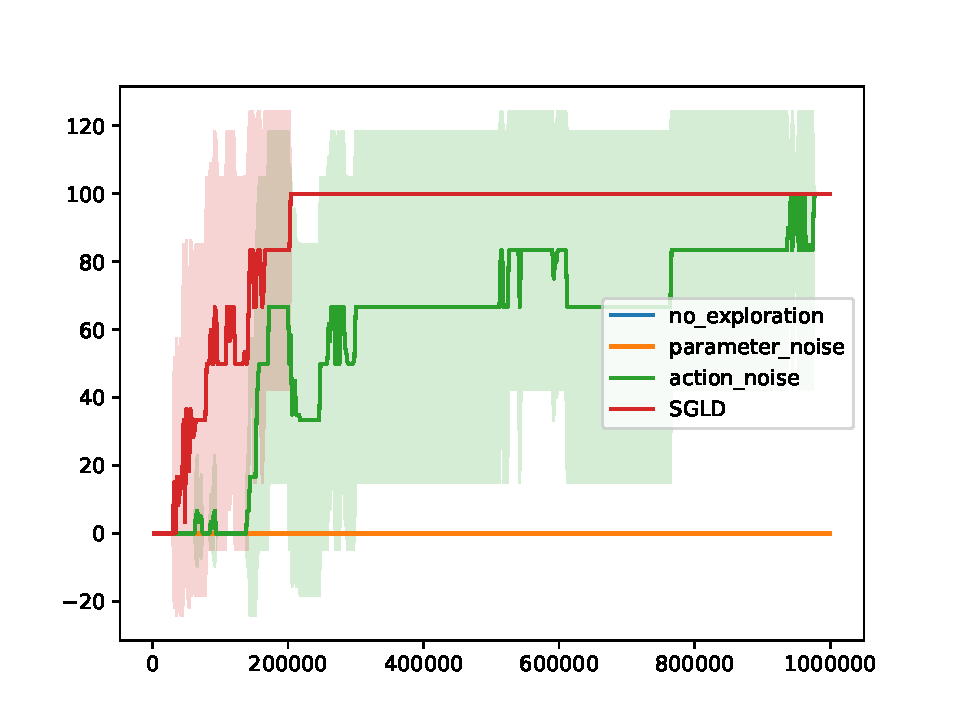
\includegraphics[width=210pt]{figs/MC0.pdf}}
      \subfigure[$\alpha = 0.1$]{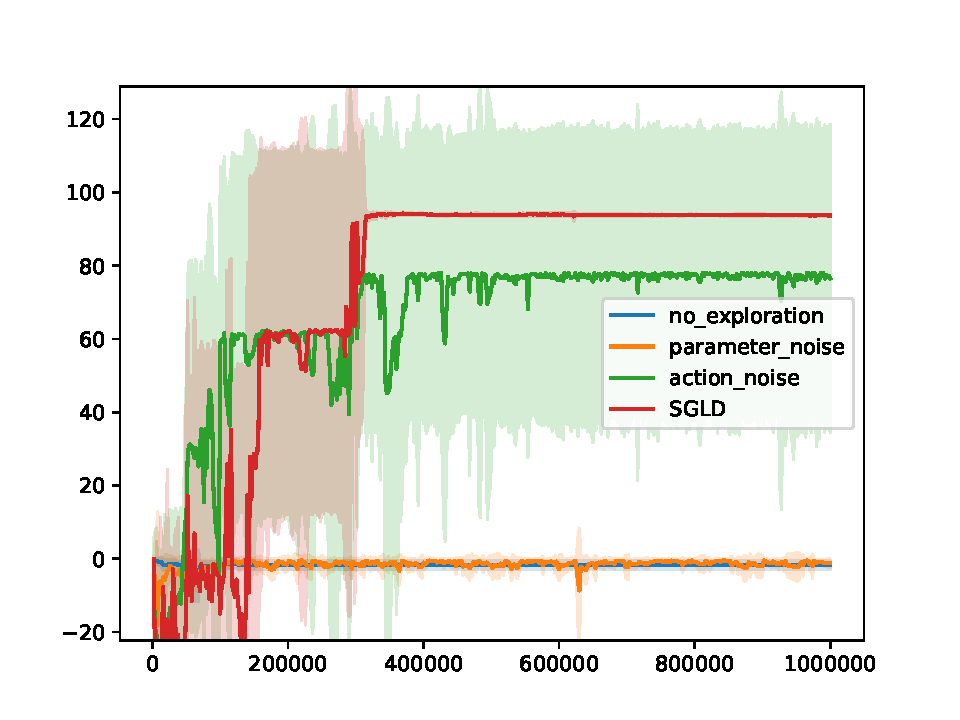
\includegraphics[width=210pt]{figs/MC.pdf}}
      \subfigure[$\alpha = 0.2$]{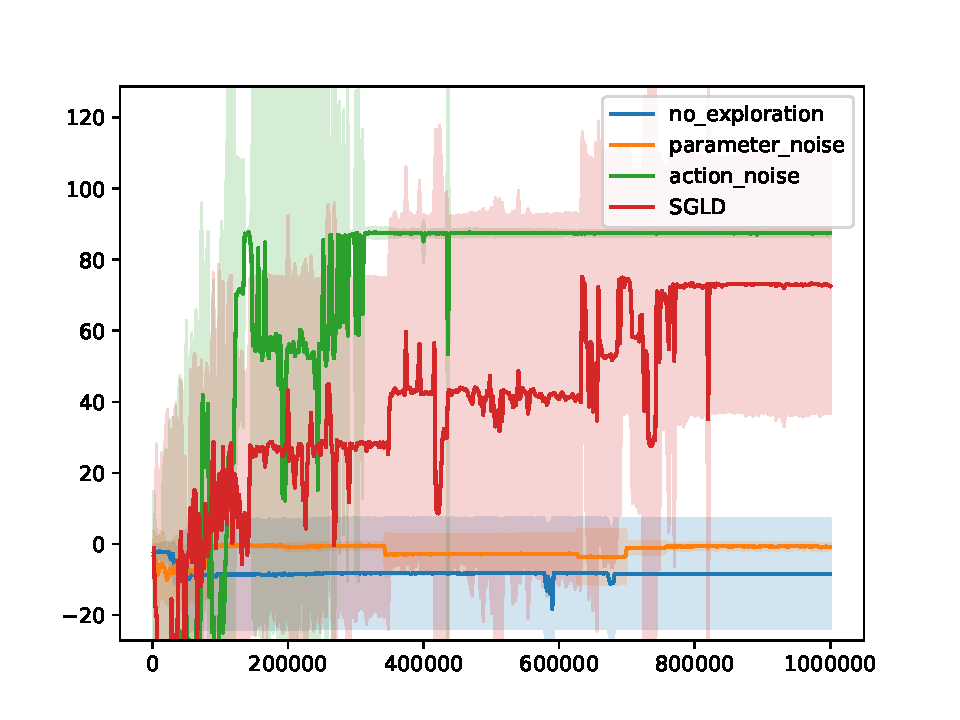
\includegraphics[width=210pt]{figs/MC0_2.pdf}}
      \subfigure[$\alpha = 0.5$]{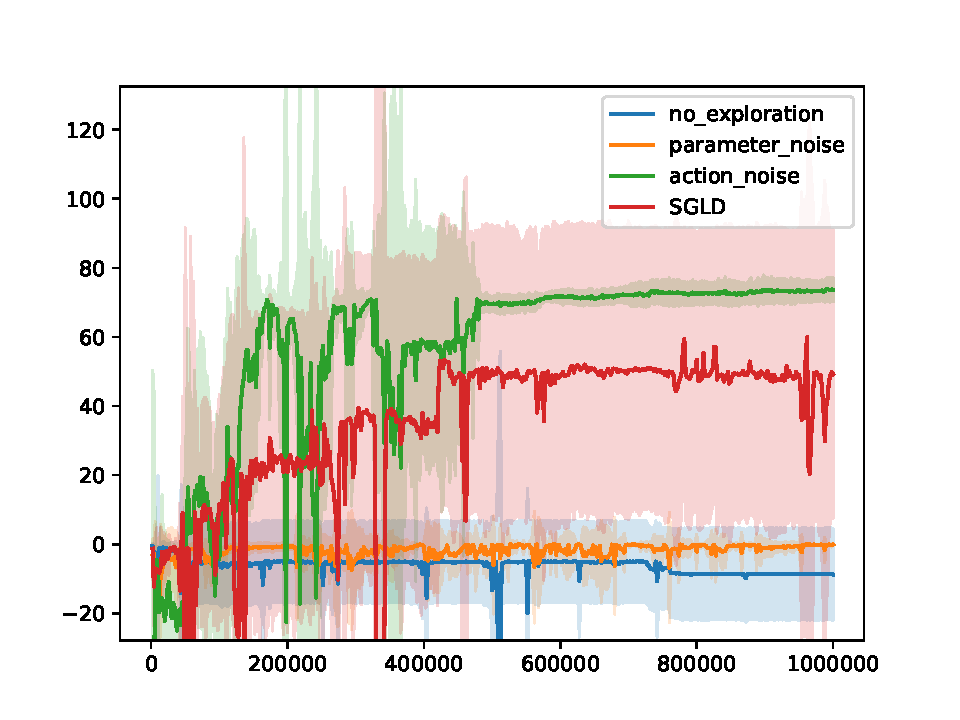
\includegraphics[width=210pt]{figs/MC0_5.pdf}}
      \subfigure[$\alpha = 1$]{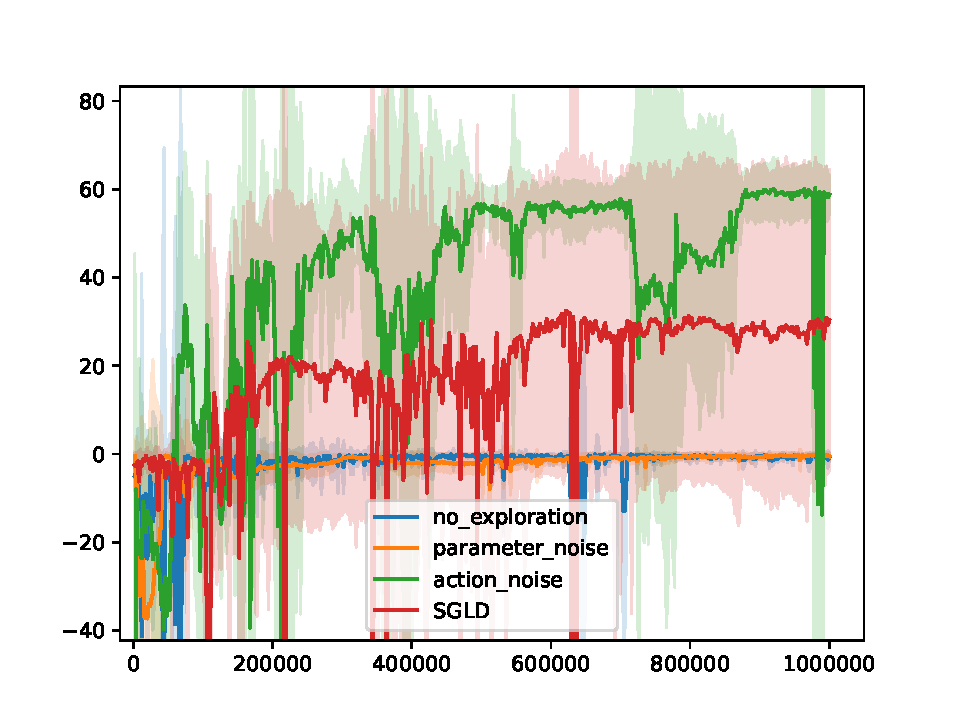
\includegraphics[width=210pt]{figs/MC1.pdf}}
   \label{fig:MCfigure}   
   \caption{MountainCar, $\alpha$ is the action penalty coefficient.}
\end{figure*}
\begin{figure*}[htb]
   \centering
      \subfigure[$\alpha = 0$]{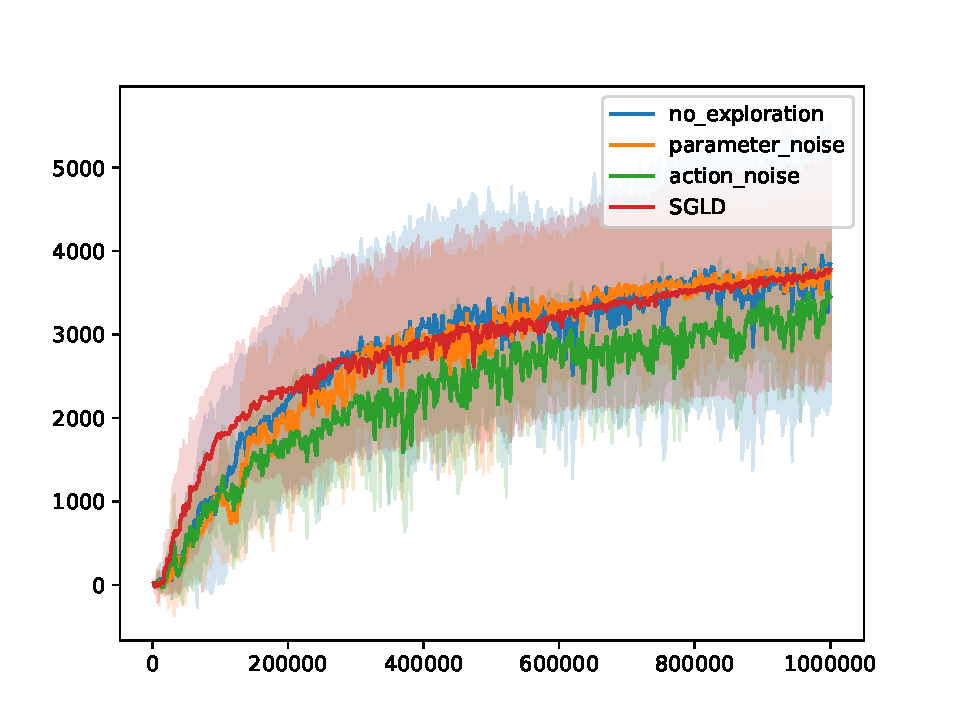
\includegraphics[width=210pt]{figs/HC0.pdf}}
      \subfigure[$\alpha = 0.1$]{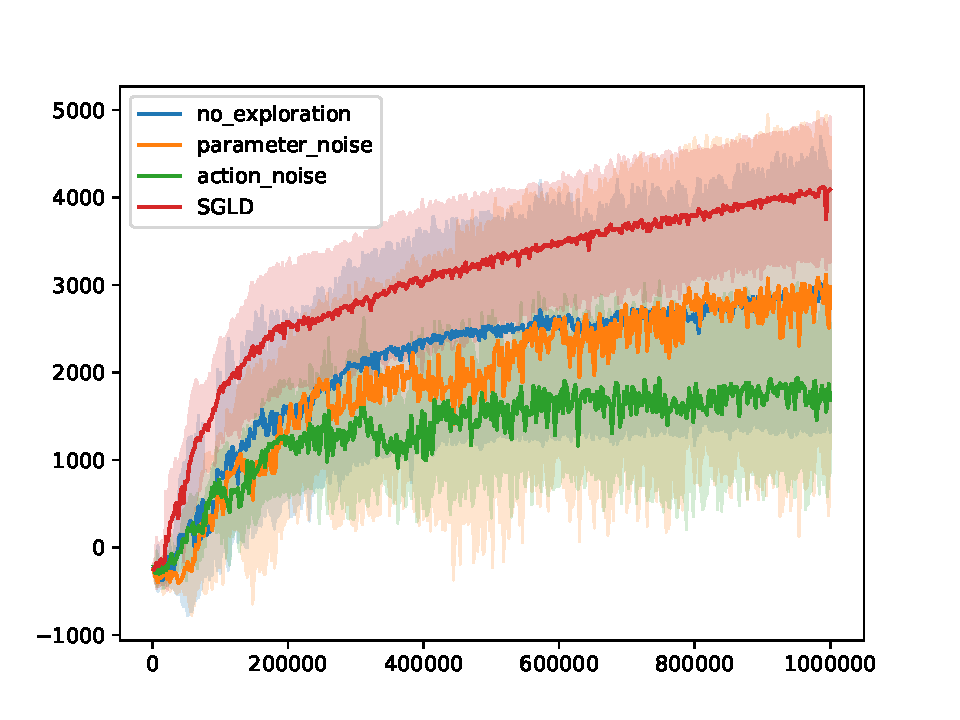
\includegraphics[width=210pt]{figs/HC.pdf}}
      \subfigure[$\alpha = 0.2$]{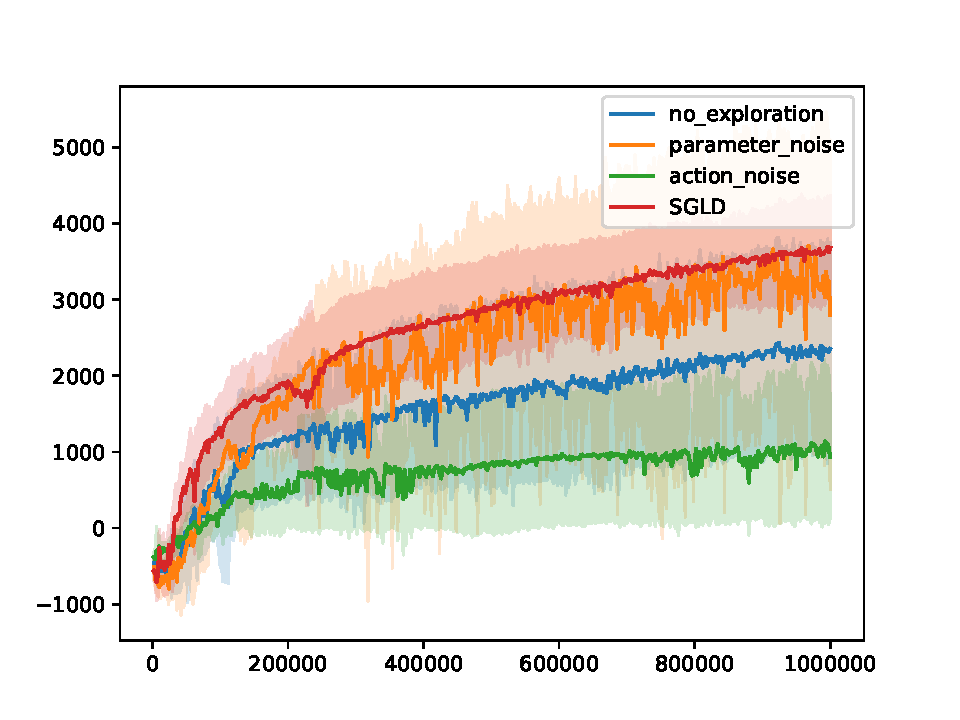
\includegraphics[width=210pt]{figs/HC0_2.pdf}}
      \subfigure[$\alpha = 0.5$]{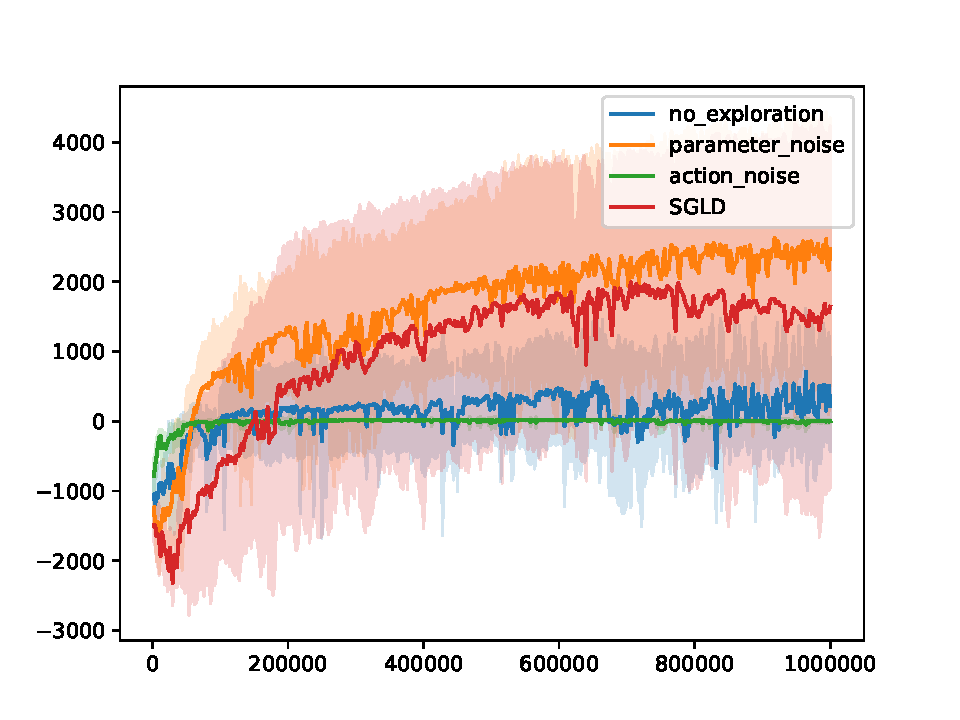
\includegraphics[width=210pt]{figs/HC0_5.pdf}}
      \subfigure[$\alpha = 1$]{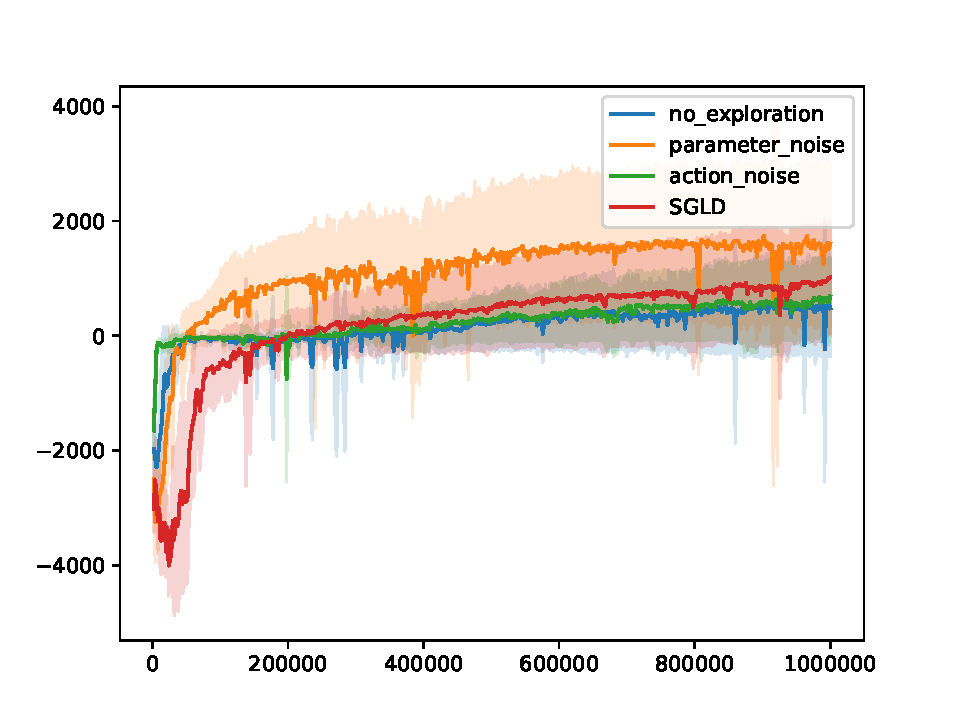
\includegraphics[width=210pt]{figs/HC1.pdf}}
   \label{fig:HCfigure}   
   \caption{HalfCheetah, $\alpha$ is the action penalty coefficient.}
\end{figure*}
\begin{figure*}[htb]
   \centering
      \subfigure[$d = 1$]{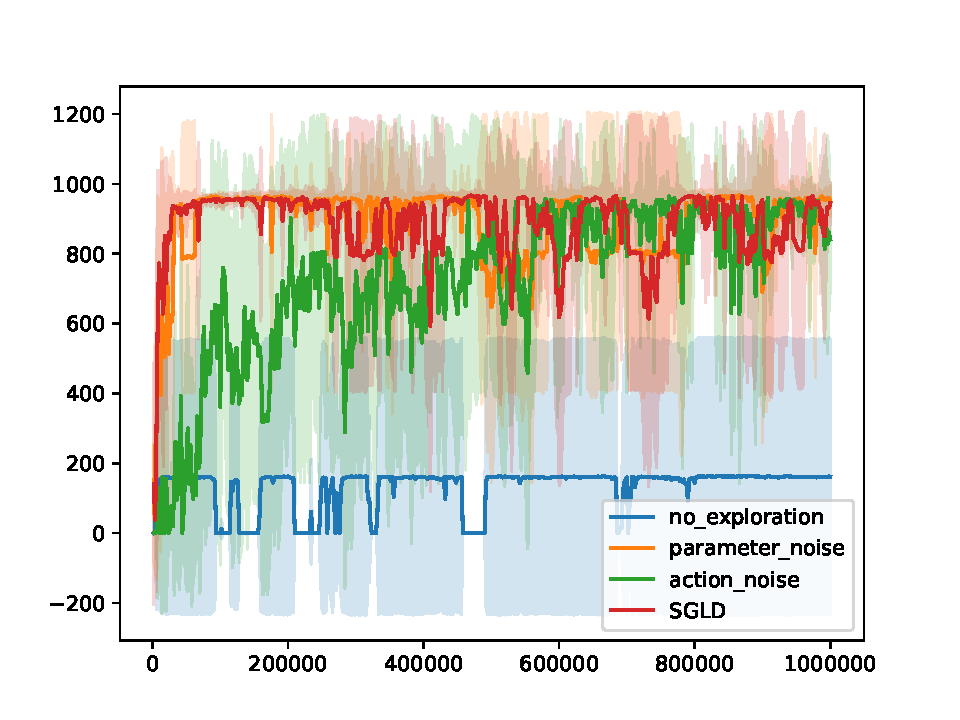
\includegraphics[width=210pt]{figs/SHC1.pdf}}
      \subfigure[$d = 2.5$]{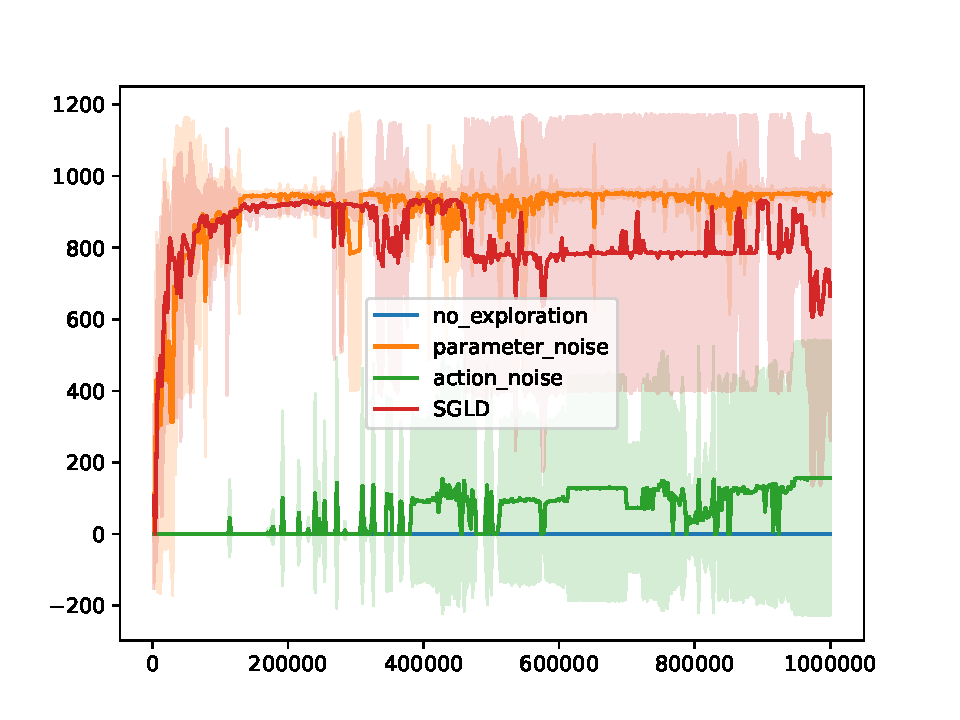
\includegraphics[width=210pt]{figs/SHC2_5.pdf}}
      \subfigure[$d = 5$]{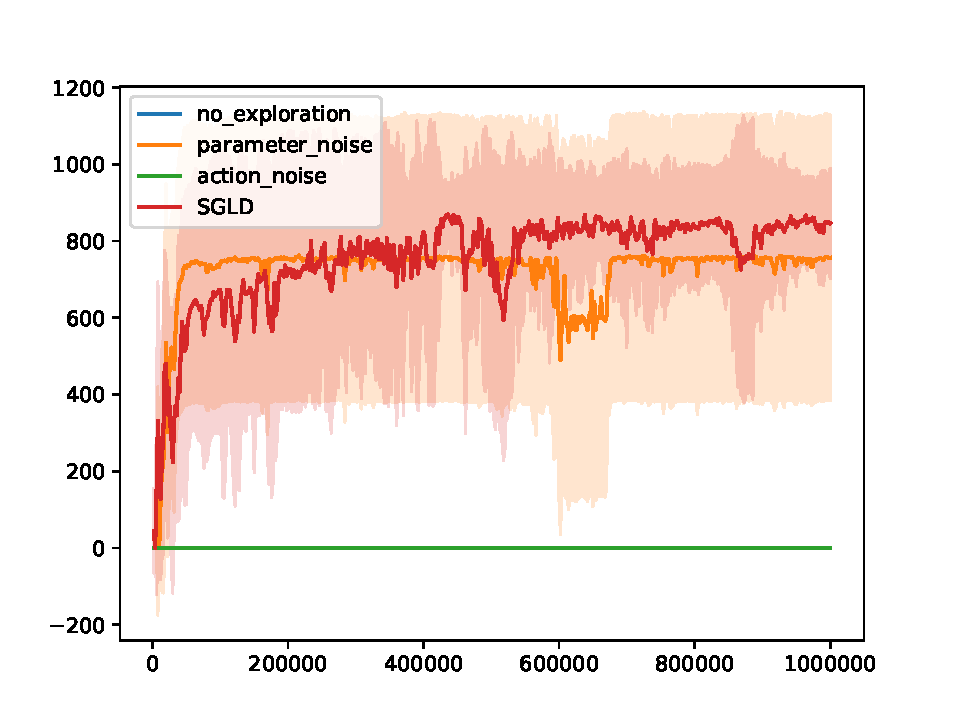
\includegraphics[width=210pt]{figs/SHC.pdf}}
      \subfigure[$d = 10$]{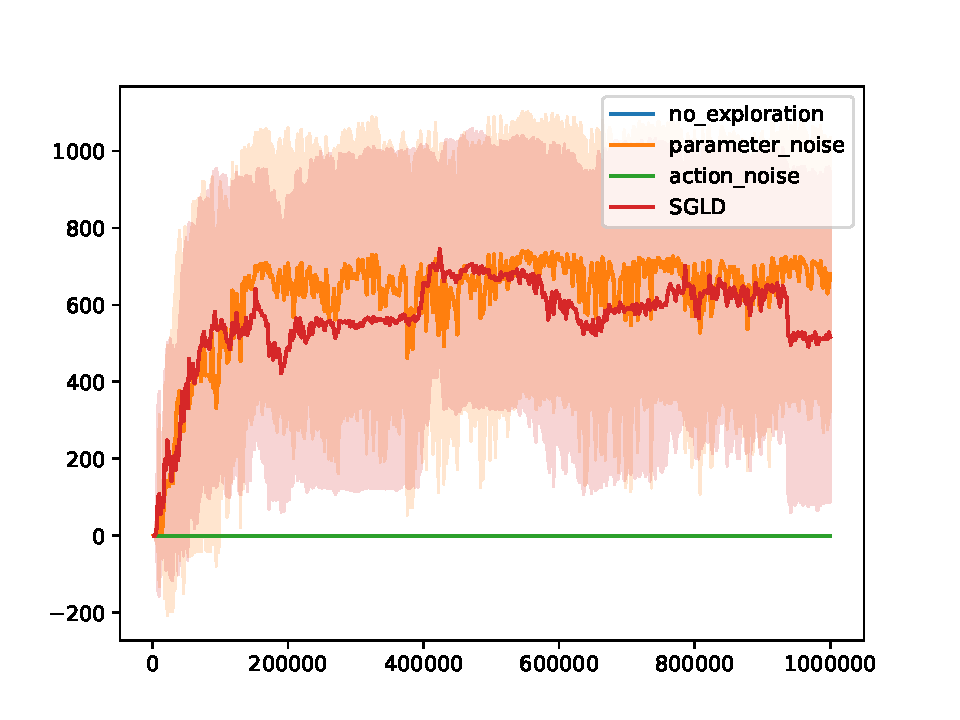
\includegraphics[width=210pt]{figs/SHC10.pdf}}
      \subfigure[$d = 20$]{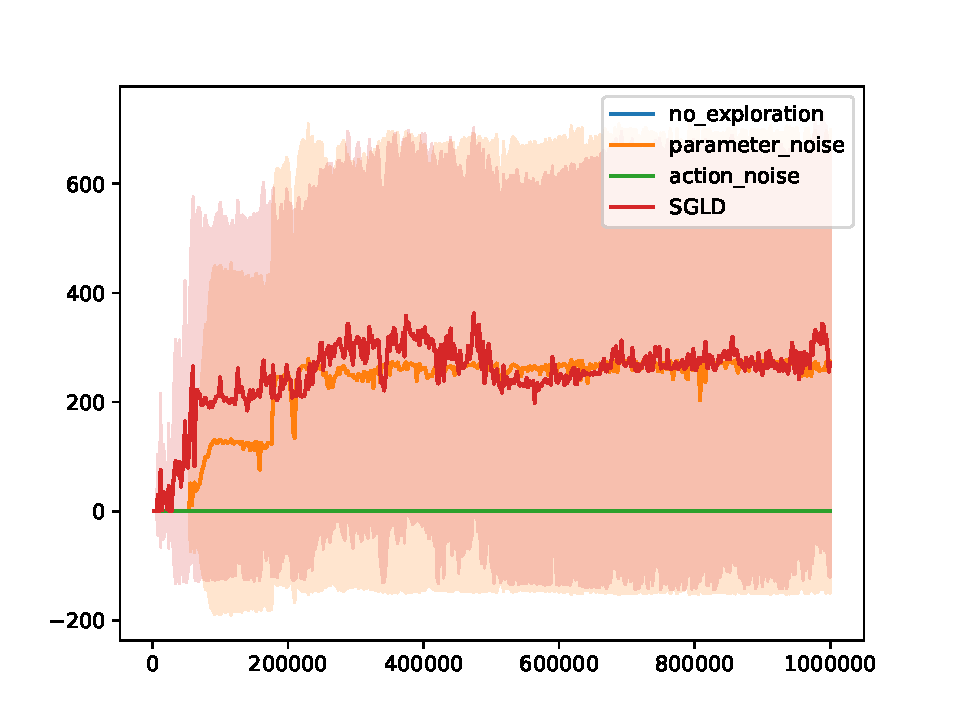
\includegraphics[width=210pt]{figs/SHC20.pdf}}
   \label{fig:SHCfigure}   
   \caption{Sparse HalfCheetah, $d$ is the distance between starting point and the finish line.}
\end{figure*}




